\section{Lecture 19 - 10/21/2022}

\subsection{Working with conformal maps}

We have described all LFTs from $\mathbb{D}$ to $\mathbb{D}$ and from $C_+$ to $\mathbb{D}$. It turns out that, if there exists a conformal map $f: \Omega \to \Dbb$, then we can describe all conformal maps to $\Dbb$! In fact, they are of the form
\[g \circ f, g: \Dbb \to \Dbb \text{ is a conformal map}\]
This is because for any two conformal maps $f_1, f_2: \Omega \to \Dbb$, $f_1 \circ f_2^{-1}$ is a conformal automorphism of the unit disk.\\\\

Now we will list some examples of conformal maps:
\begin{itemize}
    \item How can we construct a map of the following:
    \[\fbox{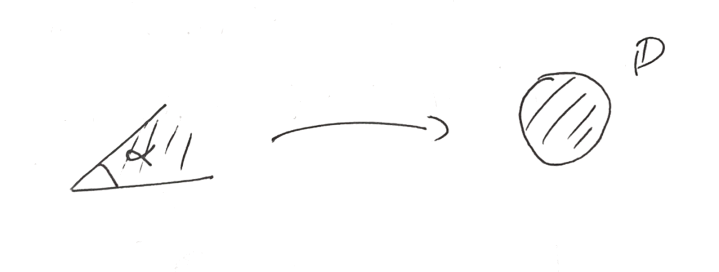
\includegraphics[width=.5\textwidth]{Figures/angle-to-disk.png}}\]
    Then consider the map $z \mapsto z^{\pi/\alpha}$ from the trianlge, this will be a conformal map onto $C_+$! Then we can pick any map from $C_+$ to $\Dbb$.
    \item Here's a map from the strip to $\mathbb{D}$:
    \[\fbox{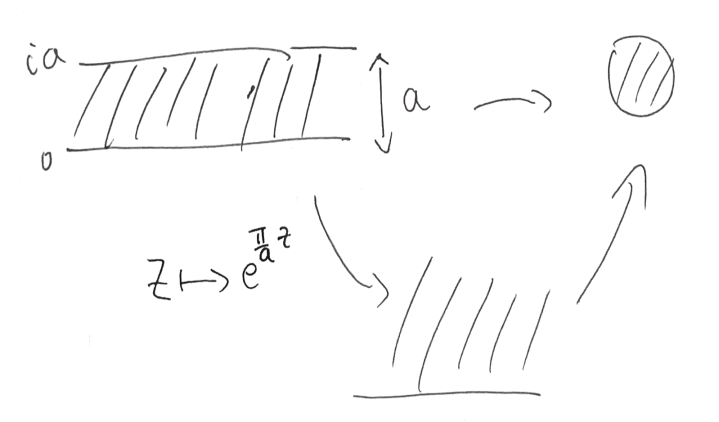
\includegraphics[width=.5\textwidth]{Figures/strip-to-disk.png}}\]
\end{itemize}

Another useful map is \textbf{Zhukovsky's function:}
    \[\varphi(z) = z + \frac{1}{z}\]
This is not an injective map! But the image of $\Dbb \cup cl(\Dbb)^c$ is the complement of $[-2, 2]$ in $\Cbb$. This is really important in aerodynamics.\\\\

There's also a conformal map from polygons into the unit disk. This is given by a formula called the \textbf{Cristoffel-Schwarz Formulas}.

\subsection{Conformally invariant metric and Hyperbolic Geometry}

\begin{definition}
    A Riemannian Manifold is a smooth manifold $M$ equipped with a metric tensor $g_{jk}$ such that the quadratic form:
    \[\sum_{j, k = 1}^n  g_{jk} x_j x_k > 0\]
    and $g_{jk} = g_{kj}$. In other words, the metric tensor is a positive definite matrix.
\end{definition}

\begin{definition}
    Suppose $\gamma: [a, b] \to M$ is a $C^1$-path, then we define the \textbf{length} of $\gamma$ as
    \[\text{Length} \gamma = \int_a^b [\sum_{j,k = 1}^n a_{j, k} (\gamma(t)) \gamma_j^'(t) \gamma_k^'(t)]^{1/2} dt\]
    Locally the metric tensor becomes quadratic form.
\end{definition}

\begin{definition}
    Let $x, y \in M$, then we define
    \[d(x, y) = \inf \{\text{Length} \gamma\ |\ \gamma \text{ connects } x, y\}\]
\end{definition}

Now for our set up in Complex Analysis, we will consider the $2$-dimensional manifold $\Dbb$. We want to find a ``conformally invariant" Riemannian Metric on $\Dbb$, in other words the metric tensor is preserved under conformal automorphisms on $\Dbb$.\\\\

What are the LFTs on $\Dbb$? We proved last lecture that they are of the form:
\[\varphi(z) = \alpha \cdot \frac{z - z_0}{1 - \overline{z_0} z}\]
We can use this to compute the metric tensor!

\begin{proof}[Computation]
    In $2$-dimension, our metric tensor is really just a $2 \times 2$ matrix, so we only need to find $4$ elements. A $2$-dimensional quadratic form is either a disk or an ellipse, and ellipse are not perserved under LFTs (think rotation).\\\\
    We will first compute the quadratic form at $z = x + iy = 0$ ($x = y = 0$), then since we know the quadratic form geometrically is a disk:
    \[(g_{jk}(0))_{j, k = 1}^2 = a^2 \begin{pmatrix}
        1 & 0\\
        0 & 1
    \end{pmatrix}\]
    So we can write the metric tensor at $z = 0$ as $M(0, dx, dy)$ (at $z = 0$)
    \[M(0, dx, dy) = a^2 ((dx)^2 + (dy)^2) = a^2 |dz|^2\]
    In particular, $dx = (\gamma_x^'), dy = (\gamma_y^')$. Now consider the Linear Transformation, 
    \[w = \frac{z - z_0}{1 - \overline{z_0} z}\]
    Then by Conformal Invariance,
    \begin{align*}
        M(z_0, dz) &= M(0, dw)\\
        &= a^2 |dw|^2\\
        &= a^2 |w'(z_0)|^2 |dz|^2 \tag*{Change of variables}
    \end{align*}
    In particular,
    \[w'(z) = (\frac{z - z_0}{1 - \overline{z_0} z})' = ... = \frac{1 - |z_0|^2}{(1 - \overline{z_0} z)^2}\]
    \[w'(z_0) = \frac{1}{1 - |z_0|^2}\]
    Hence we have that
    \[M(z_0, dz) =  (\frac{a}{1 - |z_0|^2})^2 |dz|^2\]
    It remains for us to find a suitable choice of $a$, we will choose $a = 2$. This is because
    \[\frac{2}{1 - |z_0|^2} = \frac{2}{1 + |z_0|} \cdot \frac{1}{1 - |z_0|}\]
    Note as we take the limit $|z_0| \to 1$, $\frac{2}{1 + |z_0|} $ goes to $1$ and $\frac{1}{1 - |z_0|}$ is just the inverse of the distance to the boundary.
\end{proof}

What we have just discovered is what's so called the \textbf{Hyperbolic Metric}!

\begin{definition}
    Under the hyperbolic metric, take $\gamma: [a, b] \to \Dbb$, then
    \[\text{Length}(\gamma) = \int_a^b \frac{2 |\gamma'(t)|}{1 - |\gamma(t)|^2} dt\]
\end{definition}

\begin{example}
    Take $\gamma(t) = t$, $0 \leq t \leq r < 1$, then
    \begin{align*}
        \text{Length}(\gamma) &= \int_0^r \frac{2 dx}{1 - x^2}\\
        &= \int_0^r (\frac{1}{1 - x} + \frac{1}{1 + x}) dx\\
        &= \ln(1 + r) - \ln(1 - r)\\
        &= \ln(\frac{1 + r}{1 - r})
    \end{align*}
\end{example}

It is a good exercise to show that $[0, r]$ is the shortest path from $z = 0$ to $z = r$! Then by Conformal Invariance (rotation in particular), we have that:

\begin{proposition}
    Let $z \in \Dbb$ with $|z| = r$, then
    \[dist(0, z) = \ln(\frac{1 + r}{1 - r})\]
\end{proposition}

How do we compute the distance between two points in general?

\begin{proposition}
    Let $z, w \in \Dbb$, then
    \[dist(z, w)\]
\end{proposition}

\begin{proof}
    We will use conformal invariance! Consider
    \[\varphi(\xi) = \frac{\xi - w}{1 - \overline{w} \xi} \cdot \alpha\]
    Then we have that
    \begin{itemize}
        \item $\varphi(w) = 0$
        \item $\varphi(z) = \frac{z - w}{1 - \overline{w} z} \cdot \alpha$
    \end{itemize}
    Now let
    \[\rho(z, w) \coloneqq |\frac{z - w}{1 - \overline{w} z}|\]
    We pick $\alpha$ such that $\varphi(z) = \rho(z, w)$, then 
    \[dist(z, w) = \ln(\frac{1 + \rho(z, w)}{1 - \rho(z, w)})\]
\end{proof}

\begin{definition}
    The quantity
    \[\rho(z, w) \coloneqq |\frac{z - w}{1 - \overline{w} z}|\]
    is called the \textbf{pseudohyperbolic distance}. If $\rho(z, w)$ is small (ie. $|z - w| << (1 - |z|), (1 - |w|)$, it is approximately the same as the $dist(z, w)$.
\end{definition}

In practice, what are the geodesics of the hyperbolic metric?
\begin{itemize}
    \item Any diameter through $0$ are geodesics
    \item All other geodesics are conformal images of the diameter, so they have to be circles that cross $\partial \Dbb$ perpendicularly.
\end{itemize}

\begin{remark}
    In the hyperbolic geometry on $\Dbb$, the geodesics are called ``lines". Take a link $L$ and consider $z_0 \notin L$, then there exists infinitely many ``lines" through $z_0$ that are parallel to $L$ (ie. the parallel line need not be unique).
\end{remark}

There's also a way to define Hyperbolic Geometry on the upper complex plane $\Cbb_+$, in which we define
\[M(z, dz) = |\frac{1}{Im(z)} dz|^2 \]
which is the inverse distance from point $z$ to the boundary.